\section{Design Process or Methodology Overview}
The primary objective of this research is to construct a unified, lightweight, and edge-deployable multi-task deep learning framework capable of performing four cattle monitoring tasks using image and video inputs: Body Condition Scoring (BCS), Behavior Recognition, Lameness Detection, and Cow Identification (ID). The design process follows a sequential workflow structured to mitigate task interference while maximizing parameter sharing. An overview of the proposed multi-task architecture is illustrated in Figure~\ref{fig:methodology_overview}.

\begin{figure}[h]
    \centering
    
\includegraphics[width=0.95\textwidth]{mtl_architecture.png}
    \caption{Conceptual Overview of the Multi-Task Cattle Health and Behavior Monitoring Framework.}
    \label{fig:methodology_overview}
\end{figure}

The pipeline is split into three main segments:
\begin{enumerate}
    \item \textbf{Cattle Detection and Cropping:} YOLOv8-Nano is applied to locate the cow and extract its bounding box crop, eliminating background farm clutter and normalizing the input.
    \item \textbf{Feature Extraction:} The cropped images or sequences are processed by a shared EfficientNet-B0 \cite{efficientnet2019} encoder enhanced with a Convolutional Block Attention Module (CBAM) \cite{cbam2018} to spotlight key anatomical indicators.
    \item \textbf{Task Prediction:} The feature vectors are fed into task-specific heads: ordinal regression for BCS, focal-loss classification \cite{focalloss2017} for Behavior, sequence-based LSTM for Lameness, and classification for Cow ID.
\end{enumerate}

\section{Data Collection and Preprocessing}
To establish a more transparent and reproducibility-oriented framework, using public datasets and documented preprocessing/splits, only publicly available cattle datasets were utilized. Each dataset corresponds to a specific health task.

\subsection{Dataset Profiles}
\begin{itemize}
    \item \textbf{ScienceDB BCS Dataset \cite{sciencedb2024}:} This dataset contains 53,566 high-resolution RGB images of dairy cows captured from a rear-view angle. The body condition scores are annotated using a 5-point scale with increments of 0.25. The five classes are: $\{3.25, 3.50, 3.75, 4.00, 4.25\}$.
    \item \textbf{Dryad BCS Dataset \cite{dryad2023bcs}:} 5,923 rear-view images taken in the Depth Grayscale Edge (DGE) format are included in this dataset, which combines grayscale intensity, depth coordinates, and Canny edge maps as three channels. The annotations range from integer scores of 2 to 6, representing five different ordinal classes. Moreover, this dataset includes breed and domain variety, instead of being limited only to dairy cows or Holstein cohorts.
    \item \textbf{MmCows Behavior Dataset \cite{vu2024mmcows}:} Introduced by Vu et al.~\cite{vu2024mmcows} and accessed through \cite{mmcows2024}, this dataset consists of 213,686 cropped frames obtained from continuous farm surveillance videos. The frames are labeled into seven behavior classes in this dataset: walking, standing, feeding head up, feeding head down, licking, drinking, and lying.
    \item \textbf{CattleLameness Dataset \cite{cattlelameness2024}:} Consists of side-view video clips of cows while walking. For spatiotemporal sequence modeling we compiled 50 videos, among which 25 are labeled as Lame and 25 as Normal/Sound.
    \item \textbf{OpenCows2020 Dataset \cite{opencows2020}:} Contains 4,736 images of cows labeled according to their unique individual identity across 46 classes, allowing biometrics based on vision.
    \item \textbf{CBVD-5 Dataset \cite{li2024cbvd5}:} Used exclusively as an independent test set for behavior, consisting of 2,000 balanced images of cattle behaviors to evaluate model generalization under domain shift. CBVD-5 contains five behaviors: standing, lying down, foraging, rumination, and drinking. Since our evaluation uses ``Feeding'', foraging was mapped to feeding, resulting in 4 overlapping classes (Standing, Feeding, Drinking, Lying) to match our taxonomy.
\end{itemize}

\subsection{Preprocessing Standardizations}
To ensure the deep learning models do not learn artifact features or identity shortcuts, rigorous preprocessing was applied:
\begin{itemize}
    \item \textbf{Task-Specific Splitting:} Splitting method was dependent on task. We used a cow-wise group split (unique cow IDs divided 70/15/15) for BCS and behavior recognition, to ensure that no individual cow appearing in the test set was present during training, preventing identity shortcuts. For lameness, we used a video-wise split so that no video was shared across sets. An image-wise split was performed within each identity for individual identification, where the model must identify individuals it already knows: every cow appears in train, validation, and test sets, but no individual image is shared across them.
    \item \textbf{Sparse Temporal Sampling:} Frame length varies in videos. Each video was divided into 20 equal temporal segments in order to prepare sequences for the recurrent layers while avoiding hidden-state drift and out-of-memory (OOM) GPU crashes. Then exactly one frame was selected from the center of every segment. This generated a standardized input sequence tensor with a fixed shape of $(20, 3, 224, 224)$. This sparse temporal sampling strategy is visually illustrated in Figure~\ref{fig:temporal_sampling}.

    \begin{figure}[H]
    \centering
    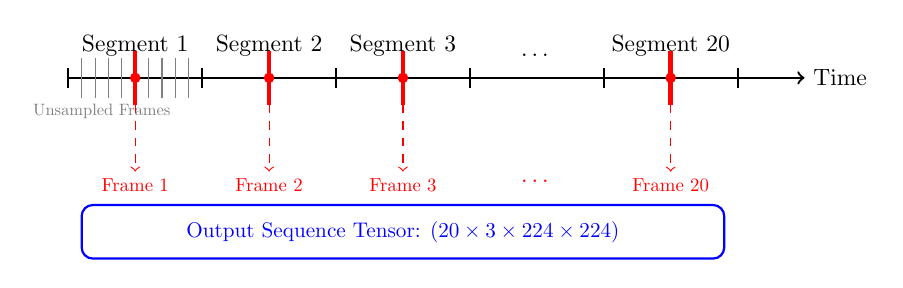
\begin{tikzpicture}[scale=0.85, every node/.style={transform shape}]
        % Draw timeline bar
        \draw[thick, ->] (0,0) -- (11.0,0) node[right] {Time};
        
        % Draw segment boundaries
        \draw[thick] (0,-0.15) -- (0,0.15);
        \draw[thick] (2,-0.15) -- (2,0.15);
        \draw[thick] (4,-0.15) -- (4,0.15);
        \draw[thick] (6,-0.15) -- (6,0.15);
        \draw[thick] (8,-0.15) -- (8,0.15);
        \draw[thick] (10,-0.15) -- (10,0.15);
        
        % Labels for segments
        \node[above] at (1,0.2) {Segment 1};
        \node[above] at (3,0.2) {Segment 2};
        \node[above] at (5,0.2) {Segment 3};
        \node[above] at (7,0.2) {\dots};
        \node[above] at (9,0.2) {Segment 20};
        
        % Draw frames as tick marks inside Segment 1 to illustrate sampling
        \foreach \f in {0.2, 0.4, 0.6, 0.8, 1.2, 1.4, 1.6, 1.8} {
            \draw[gray, thin] (\f, -0.3) -- (\f, 0.3);
        }
        \node[below, gray, scale=0.7] at (0.5,-0.3) {Unsampled Frames};
        
        % Draw center sampled frames in red
        \foreach \center/\num in {1/1, 3/2, 5/3, 9/20} {
            \draw[red, ultra thick] (\center, -0.4) -- (\center, 0.4);
            \draw[red, fill=red] (\center,0) circle (0.07);
            \draw[red, dashed, ->] (\center,-0.4) -- (\center,-1.4);
            \node[below, red, scale=0.8] at (\center,-1.4) {Frame \num};
        }
        \node[below, red] at (7,-1.4) {\dots};
        
        % Box enclosing the sequence tensor
        \draw[thick, blue, rounded corners] (0.2,-2.7) rectangle (9.8,-1.9);
        \node[blue, scale=0.9] at (5,-2.3) {Output Sequence Tensor: $(20 \times 3 \times 224 \times 224)$};
        
    \end{tikzpicture}
    \caption{Sparse Temporal Sampling illustration. The video clip is divided into 20 equal temporal segments, and exactly the center frame of each segment is sampled to construct a standardized sequence tensor of shape $(20, 3, 224, 224)$.}
    \label{fig:temporal_sampling}
    \end{figure}
    \item \textbf{Imbalance Data Capping:} The MmCows behavior dataset has a severe class imbalance. For example, lying and standing classes had more than 70,000 images, on the other hand, licking had only 2,009 images. Training directly on this results in majority-class bias. Majority classes were capped at a maximum of 3,000 randomly selected training images per epoch to reduce this problem. This resulted in a balanced sub-dataset consisting of approximately 21,000 images.
    \item \textbf{Augmentations:} Training samples were resized to $224 \times 224$ pixels, normalized using ImageNet statistics (mean=[0.485, 0.456, 0.406], std=[0.229, 0.224, 0.225]), and augmented with random horizontal flips ($p=0.5$) and random rotations ($\pm 15^\circ$). Validation and test samples were resized and normalized without augmentations.
\end{itemize}

\section{Model Architecture and Specification}
The architecture utilizes a shared parameter structure to maximize computational efficiency on edge devices.

\subsection{Shared Backbone Encoder}
The encoder backbone is initialized with ImageNet-pretrained weights from timm:
\begin{equation}
    F_{\text{raw}} = \text{Encoder}(X) \quad F_{\text{raw}} \in \mathbb{R}^{B \times C \times H \times W}
\end{equation}
EfficientNet-B0 \cite{efficientnet2019} (5.3M parameters) and MobileNetV3-Small \cite{mobilenetv3} (2.5M parameters) were evaluated, with EfficientNet-B0 selected as the final backbone due to its superior feature representation.

\subsection{CBAM Attention Module}
A Convolutional Block Attention Module (CBAM) \cite{cbam2018} is inserted immediately after the backbone's final feature map.
\begin{itemize}
    \item \textbf{Channel Attention:} Identifies ``what'' channels contain relevant signal using average and max pooling:
    \begin{equation}
        M_c(F) = \sigma(\text{MLP}(\text{AvgPool}(F)) + \text{MLP}(\text{MaxPool}(F)))
    \end{equation}
    \item \textbf{Spatial Attention:} Highlights ``where'' the relevant anatomy lies (e.g. spine line for BCS, joint positions for lameness) using a $7 \times 7$ convolution over channel-concatenated maps:
    \begin{equation}
        M_s(F') = \sigma(f^{7 \times 7}([\text{AvgPool}(F'); \text{MaxPool}(F')]))
    \end{equation}
\end{itemize}
The final attention-weighted feature map is pooled using Adaptive Average Pooling and flattened to a 1,280-dimensional feature vector.

\subsection{Task-Specific Prediction Heads}
The feature vector is routed to four independent task heads:
\begin{enumerate}
    \item \textbf{BCS Head:} A linear layer projecting the 1,280 features to 4 outputs representing the ordinal ranking.
    \item \textbf{Behavior Head:} A linear classification layer projecting the 1,280 features to 7 behavior logits for frame-level prediction. In the spatiotemporal multi-task configuration, the sequence of feature vectors is processed through the shared LSTM pathway before classification. For behavior recognition, temporal sequences were constructed by grouping consecutive sampled MmCows frames from the same cow/video segment before passing features to the LSTM.
    \item \textbf{Lameness Head (Temporal LSTM):} The sequence of 20 feature vectors is processed by a single-layer LSTM (hidden size = 256, dropout = 0.5), followed by a linear classification layer to output a binary logit.
    \item \textbf{Cow ID Head:} A linear layer projecting features to $N$ cattle identity classes.
\end{enumerate}

\section{Loss Functions and Optimizations}
Each task is optimized using a loss function tailored to its specific mathematical properties:

\subsection{Consistent Rank Logits (CORAL) Loss for BCS}
To preserve the natural ordering of body condition scores, ordinal regression using the Consistent Rank Logits (CORAL) framework \cite{coral2020} was formulated. For $K$ classes (where $K=5$), the model outputs $K-1=4$ binary logits. The loss is computed as the sum of binary cross-entropies:
\begin{equation}
    L_{\text{BCS}} = -\frac{1}{K-1} \sum_{i=1}^{K-1} \left[ y_i \log(\sigma(g_i)) + (1 - y_i) \log(1 - \sigma(g_i)) \right]
\end{equation}
where $y_i = \mathbb{I}(y > i)$ is the binary rank representation of the actual score. Predictions are computed by summing the sigmoid outputs:
\begin{equation}
    \hat{y} = \sum_{i=1}^{K-1} \mathbb{I}(\sigma(g_i) > 0.5)
\end{equation}

\subsection{Focal Loss for Behavior Classification}
To prevent the overwhelming majority classes from dominating training gradients, Focal Loss \cite{focalloss2017} is applied to the behavior outputs:
\begin{equation}
    L_{\text{Behavior}} = -\alpha_t (1 - p_t)^\gamma \log(p_t)
\end{equation}
where $p_t$ is the model's estimated probability for the correct class, $\alpha_t = 0.25$ is applied as a uniform scalar balancing factor (rather than a per-class weight vector, representing a simplification), and $\gamma = 2.0$ is the focusing parameter that down-weights easy, well-classified examples.

\subsection{Lameness and ID Losses}
Binary Cross-Entropy (BCE) with logits loss is utilized for the binary lameness classification task:
\begin{equation}
    L_{\text{Lameness}} = - \left[ y \log(\sigma(x)) + (1-y) \log(1-\sigma(x)) \right]
\end{equation}
Standard Cross-Entropy Loss with Softmax normalization is utilized for individual cow identification:
\begin{equation}
    L_{\text{ID}} = - \sum_{c=1}^N y_c \log(\text{Softmax}(x_c))
\end{equation}

\section{Implementation of Selected Design and Training Strategy}
The training pipeline was executed on PyTorch using a phased sequential training methodology to avoid destructive task interference (where gradient updates for one task corrupt the weights learned for another).

\subsection{Reproducibility Configuration}
All experiments were conducted with a single run using the default PyTorch random seed. Standard deviation across multiple runs was not computed due to the computational cost of the six-phase training pipeline. This represents a limitation: all reported metrics are point estimates without confidence intervals. Furthermore, we evaluated exclusively on public datasets to support a more transparent and reproducibility-oriented framework. The preprocessing scripts, exact train/validation/test split configurations, and hyperparameter logs will be released in a public repository upon completion to facilitate independent verification.

\subsection{Phased Sequential Training}
\begin{itemize}
    \item \textbf{Phase 1: Encoder Initialization.} The EfficientNet-B0 backbone is initialized with ImageNet-pretrained weights.
    \item \textbf{Phase 2: BCS Head Training.} The backbone weights are frozen. The attention layer and BCS head are trained separately on the Dryad and ScienceDB datasets for 30 epochs using the Adam optimizer (lr = $10^{-3}$, scheduler decay = 0.5 every 10 epochs).
    \item \textbf{Phase 3: Behavior Head Training.} The backbone is kept frozen. The behavior head is trained for 30 epochs using Focal Loss on the capped MmCows dataset. Early stopping is monitored with a patience of 10 epochs.
    \item \textbf{Phase 4: Lameness Sequence Training.} The backbone remains frozen. Bounding box sequence crops are extracted using YOLOv8-Nano. The LSTM temporal layers and classification head are trained on 20-frame sequences for 15 epochs.
    \item \textbf{Phase 5: Cow ID Training.} The backbone remains frozen. The ID head is trained on OpenCows2020 for 10 epochs.
    \item \textbf{Phase 6: Multi-Task Joint Optimization.} All heads are attached. The backbone is unfrozen, and the model is trained end-to-end using the multi-task loss weight configuration:
    \begin{equation}
        L_{\text{total}} = 0.35 \cdot L_{\text{BCS}} + 0.35 \cdot L_{\text{Behavior}} + 0.15 \cdot L_{\text{Lameness}} + 0.15 \cdot L_{\text{ID}}
    \end{equation}
    The task weights assigned to each loss component ($0.35$ for BCS and Behavior, and $0.15$ for Lameness and ID) are determined by the relative dataset sizes and task complexities. Body Condition Scoring (BCS) and Behavior Recognition represent complex visual classification tasks backed by very large datasets (53,566 images for ScienceDB and over 21,000 capped frames for MmCows). In contrast, Lameness Detection (50 sequence samples) and Cow Identification (4,736 images) have simpler classification scopes or operate on much smaller sample registers. Assigning higher loss weights to the larger and more complex tasks prevents the shared encoder backbone from drifting and over-specializing on the smaller datasets during backpropagation. These weights were selected empirically based on relative dataset sizes and task complexities; formal sensitivity analysis comparing alternative weightings is deferred to future work.
\end{itemize}

\subsection{Live Video Inference Architecture}
During live deployment, the system processes videos frame-by-frame through a sliding window. First, the YOLOv8-Nano detector derives cattle crops. These crops are then normalized and queued. The following operations are performed once the queue contains 20 crops:
\begin{itemize}
    \item The sequence is passed through the shared encoder and LSTM, which generates a single, stable locomotion score for predicting lameness.
    \item Moreover, 20 distinct frame-level predictions are produced by the spatial heads. In order to prevent noise, temporal averaging is used to average frame-level BCS scores. Majority voting is used across the 20 frames to generate cow ID predictions. This helps reduce temporary occlusions such as background posts or dust and also ensures high deployment reliability.
\end{itemize}
